
En este capítulo se describe cómo se han aplicado los algoritmos en los tres problemas de optimización planteados, como se ha indicado en el flujo de trabajo del TFG (fig.~\ref{fig:3-esquema_disenyo}).

Se aplica QAOA al problema presentado en la página web tutorial de Qiskit~\cite{qiskit_tutorial_antiguo}.
\\
En el siguiente problema se pretende reproducir el circuito obtenido en el artículo por Urgelles \textit{et al.} (2022)\cite{multi-objective_routing_optimization}, el cual aumenta la complejidad con respecto al problema previo al añadir restricciones y aumentar el número de qubits.
\\
Debido a los resultados obtenidos en el problema anterior (\textit{sección~\ref{sec:5-primer_grafo}}), se decide aplicar las mismas pruebas sobre otro grafo con el mismo problema, para estudiar el funcionamiento del algoritmo al aumentar el número de capas.
Este es obtenido del artículo por Fan \textit{et al.} (2023)\cite{solving_shortest_path_with_qaoa}.

La implementación de QAOA ha sido realizada en código Python en cuadernos de Jupyter y se encuentra disponible en un repositorio de Github habilitado (\textit{sección~\ref{CAP:github}} del apéndice).

\begin{figure}[Esquema del algoritmo]{fig:4-esquema_algoritmo}{Esquema del algoritmo}
  \centering
  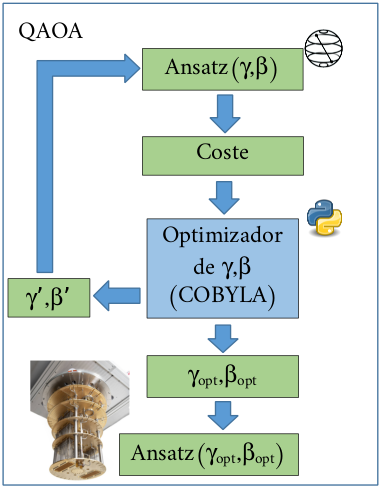
\includegraphics[scale=0.4]{esquema_algoritmo.png}
\end{figure}

En el \textit{código~\ref{cod:4-fragmento_qaoa}} se muestra un fragmento ilustrativo de la implementación del algoritmo.

\newpage

\begin{lstlisting}[language=Python,label=cod:4-fragmento_qaoa,caption={Fragmento de código de una ejecución de QAOA.},style=numbered]
def compute_expectation(counts: Dict[str, int]) -> float:
    media = 0
    for bits, count in counts.items():
        cost = eval_cost_function(bits)
        media += cost * count

    return media

def execute_circuit(theta: List[float]) -> float:
    qc = generate_qaoa_circuit(theta)
    counts = sampler.run(qc).result().quasi_dists[0].binary_probabilities()
    return compute_expectation(counts)

theta = minimize(execute_circuit, [1.0, 1.0] * num_layers, method="COBYLA")
\end{lstlisting}

La correspondencia entre el código escrito y el funcionamiento del algoritmo es el siguiente.
\\
Como ya se ha mencionado, para modificar los parámetros $\beta, \gamma$ se hace uso de un optimizador clásico llamado \textit{Constrained Optimization BY Linear Approximation} (COBYLA), perteneciente a la biblioteca \textit{scipy} (línea 14 del \textit{código~\ref{cod:4-fragmento_qaoa}}).
\\
Este realiza sucesivas llamadas a un método con una lista de floats (que corresponde a los vectores $\beta$ y $\gamma$) como entrada y un float como salida (que corresponde al valor esperado del operador $C$).
Tras cada llamada a este método se modifican los valores de entrada, con el fin de minimizar la salida (coste) obtenida.
\\
En este caso, ese método a minimizar es denominado \textit{execute\_circuit()} (línea 9 del \textit{código~\ref{cod:4-fragmento_qaoa}}) y tiene tres partes:

\begin{itemize}
\item La generación del circuito cuántico a partir del parámetro \textit{theta}, el cual corresponde con los dos vectores $\beta$ y $\gamma$ concatenados, de acuerdo con el circuito ansatz del problema, calculado previamente.
  Esto es realizado por la función \textit{generate\_qaoa\_circuit()}.
  Corresponde con el \textit{paso~\ref{it:3-algoritmo_construir_circuito}} del algoritmo.

\item La ejecución del circuito utilizando la librería de Qiskit.
    Corresponde al \textit{paso~\ref{it:3-algoritmo_ejecutar_circuito}} del algoritmo.

\item La evaluación del resultado obtenido, realizado por la función \textit{compute\_expectation(counts: Dict[str, int])} (línea 1 del \textit{código~\ref{cod:4-fragmento_qaoa}}), el cual calcula el valor esperado de $C$ de manera clásica, donde \textit{eval\_cost\_function()} devuelve el coste un valor en la función de coste QUBO\@.
  Corresponde al \textit{paso~\ref{it:3-algoritmo_valor_esperado}} del algoritmo.
\end{itemize}

Una vez se cumplan los criterios de convergencia seguidos por COBYLA, se devolverá esa entrada \textit{theta}, equivalente a $\vec{\gamma} | \vec{\beta}$, con la que se puede volver a ejecutar el circuito ansatz resultante de \textit{generate\_qaoa\_circuit()}, para lograr el resultado del algoritmo.


\section{Max-cut en grafo de 4 aristas\label{sec:4-tutorial_de_qiskit}}{desarrollo/tutorial_qiskit.tex}

\section{Camino más corto en grafo de 4 nodos\label{sec:4-primer_grafo}}{desarrollo/primer_grafo.tex}

\section{Camino más corto para estudiar la variación con el número de capas\label{sec:4-zhiqiang}}{desarrollo/zhiqiang_grafo.tex}

%%% Local Variables:
%%% mode: latex
%%% TeX-master: "../tfgtfmthesisuam"
%%% End:
